\documentclass{standalone}
\usepackage{tikz}
\usepackage{ctex,siunitx,upgreek}
\setCJKmainfont{Noto Serif CJK SC}
\usepackage{tkz-euclide}
\usepackage{amsmath}
\usetikzlibrary{patterns, calc}
\usetikzlibrary {decorations.pathmorphing, decorations.pathreplacing, decorations.shapes,}
\begin{document}
\small
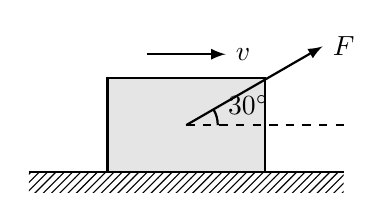
\begin{tikzpicture}[>=latex,thick,scale=1]
  \fill [pattern = north east lines] (0,-.25) rectangle (4,0);
  \draw (0,0)--(4,0);
  \draw [fill=gray!20] (1,0) rectangle (3,1.2);
  \draw [dashed] (2,0.6)--(4,0.6);
  \draw [->] (2,0.6)--++(30:2.0)node [right]{$F$};
  \draw [->] (1.5, 1.5)--(2.5,1.5) node [right]{$v$};
  \draw (2.4,0.6) arc(0:30:.4) node[at start,above right]{\ang{30}};
\end{tikzpicture}
\end{document}